% This is based on "sig-alternate.tex" V1.9 April 2009
% This file should be compiled with V2.4 of "sig-alternate.cls" April 2009
%
\documentclass{report}

\usepackage[english]{babel}
\usepackage{graphicx}
\usepackage{tabularx}
\usepackage{subfigure}
\usepackage{enumitem}
\usepackage{url}


\usepackage{color}
\definecolor{orange}{rgb}{1,0.5,0}
\definecolor{lightgray}{rgb}{.9,.9,.9}
\definecolor{java_keyword}{rgb}{0.37, 0.08, 0.25}
\definecolor{java_string}{rgb}{0.06, 0.10, 0.98}
\definecolor{java_comment}{rgb}{0.12, 0.38, 0.18}
\definecolor{java_doc}{rgb}{0.25,0.35,0.75}

% code listings

\usepackage{listings}
\lstloadlanguages{Java}
\lstset{
	language=Java,
	basicstyle=\scriptsize\ttfamily,
	backgroundcolor=\color{lightgray},
	keywordstyle=\color{java_keyword}\bfseries,
	stringstyle=\color{java_string},
	commentstyle=\color{java_comment},
	morecomment=[s][\color{java_doc}]{/**}{*/},
	tabsize=2,
	showtabs=false,
	extendedchars=true,
	showstringspaces=false,
	showspaces=false,
	breaklines=true,
	numbers=left,
	numberstyle=\tiny,
	numbersep=6pt,
	xleftmargin=3pt,
	xrightmargin=3pt,
	framexleftmargin=3pt,
	framexrightmargin=3pt,
	captionpos=b
}

% Disable single lines at the start of a paragraph (Schusterjungen)

\clubpenalty = 10000

% Disable single lines at the end of a paragraph (Hurenkinder)

\widowpenalty = 10000
\displaywidowpenalty = 10000
 
% allows for colored, easy-to-find todos

\newcommand{\todo}[1]{\textsf{\textbf{\textcolor{orange}{[[#1]]}}}}

% consistent references: use these instead of \label and \ref

\newcommand{\lsec}[1]{\label{sec:#1}}
\newcommand{\lssec}[1]{\label{ssec:#1}}
\newcommand{\lfig}[1]{\label{fig:#1}}
\newcommand{\ltab}[1]{\label{tab:#1}}
\newcommand{\rsec}[1]{Section~\ref{sec:#1}}
\newcommand{\rssec}[1]{Section~\ref{ssec:#1}}
\newcommand{\rfig}[1]{Figure~\ref{fig:#1}}
\newcommand{\rtab}[1]{Table~\ref{tab:#1}}
\newcommand{\rlst}[1]{Listing~\ref{#1}}

% General information

\title{Multiplayer Pac-Man\\
\normalsize{Distributed Systems -- Project Proposal}}
\subtitle{subtitle}

% Use the \alignauthor commands to handle the names
% and affiliations for an 'aesthetic maximum' of six authors.

\numberofauthors{1} %  in this sample file, there are a *total*
% of EIGHT authors. SIX appear on the 'first-page' (for formatting
% reasons) and the remaining two appear in the \additionalauthors section.
%
\author{
% You can go ahead and credit any number of authors here,
% e.g. one 'row of three' or two rows (consisting of one row of three
% and a second row of one, two or three).
%
% The command \alignauthor (no curly braces needed) should
% precede each author name, affiliation/snail-mail address and
% e-mail address. Additionally, tag each line of
% affiliation/address with \affaddr, and tag the
% e-mail address with \email.
%
% 1st. author
\alignauthor \normalsize{Student One,  Student Two, Linus Fessler}\\
	\affaddr{\normalsize{ETH ID-1 XX-XXX-XXX, ETH ID-2 XX-XXX-XXX, ETH ID-3 14-924-203}}\\
	\email{\normalsize{one@student.ethz.ch, two@student.ethz.ch, fesslerl@student.ethz.ch}}
}


\begin{document}

\maketitle

\section{Introduction}

%------------------------------------INTRODUCTION------------------------------------

Since 1980, the game Pac-Man has fascinated players around the world. 
Starting as an arcade game, it was adapted for many platforms while technology was improving and is still played today on mobile devices.
While graphics have improved significantly over time and new features were added to the original idea of the game, there is still a major drawback to most of its versions as the game only provides single player user experience.

 
Our goal is therefore to exploit the opportunities of modern mobile devices in order to create a new user experience. 
This new user experience will consist of the well known Pac-Man game combined with a distributed multi player approach.
The idea will be implemented as an android application allowing the user to create a new instance of the game by starting a server on an android device. 
Other users can then connect to this server with their own devices.



\section{System Overview}

%-----------------------------------SYSTEM OVERVIEW----------------------------------
Figure 1 gives an overview of the Pacman app Activities.
The app starts in the Main activity. 
Here, the user can choose to either edit the game settings, host or join a game by pressing corresponding buttons.

If the user presses the "Settings" button, the app will switch to the Settings Activity, where the devices local IP address is listed and the following properties can be changed:
\begin{enumerate}
	\item The username that will be used in the game.
	\item The port on which the local server would listen to.
	\item The IP address and port on which the app would try to connect to a server.
\end{enumerate}

If the user chooses the "Host" button, the app will switch to the Lobby Activity (Host).
Here, the user can await new clients and see which ones are currently connected (identified by usernames).
Furthermore, the user can decide to start the game by pressing a "Start" button.
This will launch the Game Activity and start the actual game.

If the user chooses the "Join" button, the app will switch to the Lobby Activity (Client).
Here, the user can see the host's username and which clients are currently connected (identified by username).
In contrast to the host's view, the client can not see a "Start" button, but instead has to wait for the host to start the game.

Independent from the device's role as host or client, the app will automatically switch to the Score Activity after the game has ended.
This Activity displays each users score (determined by the gameplay performance).
The only following action is to return to the Main Activity by pressing a button. 
 

---------------------------------------------------------------------------

Figure 1 gives an overview of the Pacman app.
The starting activity is the Main activity. 
From there the user can either choose to host a game or to join a game. 
In the former case, the user needs to specify in the Settings activity to which port should the other players connect. 
In the latter case, the user needs to configure in the Settings activity the IP address of the host and the port number of the host. 
Furthermore, before joining (or hosting) a game, the user should specify an (unique) name.

After choosing to join a game, the app will switch from the Main activity to the Lobby activity.
From there on, the user/app needs to wait for the host to start the game. Of course, if the user has not configured his/her settings appropiately (for instance, invalid port number for the host), then the app will notify the user. 
Conversely, if the user is the host, the app will make sure he has a (valid) port number. 
Moreover, it should check that all names are unique. If there is a name clash, the app can and should kick those players out. Once the host is ready, he/she can start the game.


Once the game started, a Score activity keeps track of the current performance of the players. 
If Pacman (i.e. the host) manages to take all the points that are positioned on the map, he wins the round and gets one point. 
Otherwise, if a ghost manages to capture Pacman, then the ghost gets one point. 
[??? is this the way we should keep track of the score? any other proposals?]

\begin{figure} [ht!]
	\centering
    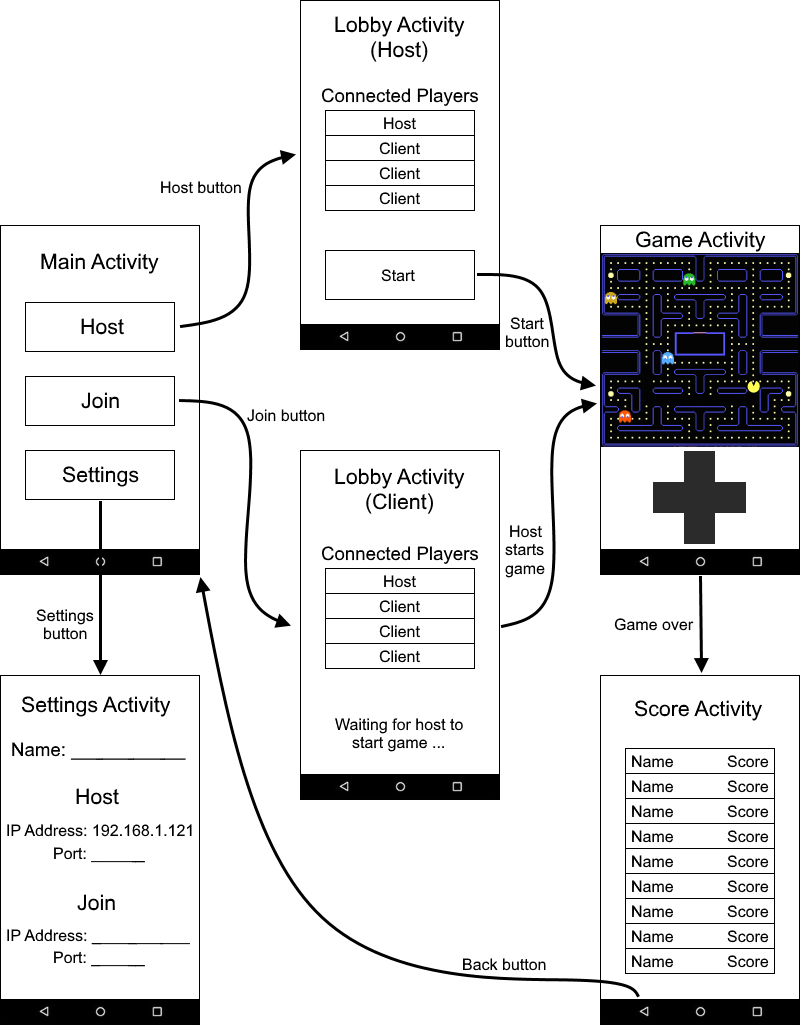
\includegraphics[width=\columnwidth]{overview.png}
    \lfig{activity-overview}
    \vspace{-5mm} % use negative white space to fix too large gaps
	\caption{Activity Overview}
\end{figure}

\section{Requirements}

%-------------------------------------REQUIREMENTS------------------------------------

\begin{enumerate}
	\item The game can be played on multiple Android devices (at least two).
	\item The gameplay should work as follows:
	\begin{enumerate}
		\item Coins are distributed evenly on the game map (board).
		\item One player plays as Pac-Man.
		\item One or multiple other players play as ghosts.
		\item Pac-Man wins, if he collects all coins on the map.
		\item The ghosts win, if they capture Pac-Man (simply modelled by collision).
	\end{enumerate}
	\item Each player must use one Android device in order to control his figure (Pac-Man or ghost).
	\item The map (board) on which the players move should provide the following features:
	\begin{enumerate}
		\item Pac-Man starts on a predefined location (Pac-Man spawn).
		\item The ghosts (one ore multiple) start on predefined locations (ghost spawns).
		\item Player figures can only move up, down, left and right.
		\item The only structuring elements of the map are walls.
		\item Walls have eiter horizontal or vertical orientation.
		\item Player figures can not move through walls.
		\item The map has rectangular shape and is limited by walls at its borders (horizontal walls along the left and right border, vertical walls along upper and bottom border).
		\item Every position at the map that is not occupied by a wall must be reachable for the player figures. 
	\end{enumerate}
	\item The protocol used for Device-to-Device communication will will be implemented atop UDP, TCP or a higher-level protocol. [???]
	\item The app will be optimized for Android version [???] and run on Android version [???] and higher. [???]
	\item The host will play as Pac-Man.
	\item Clients will play as ghosts.
	\item On the hosting player's device, a service will be started to run the server which the clients can connect to.
	\item As a game development engine the ANDEngine is used. This is a free Android 2D OpenGL game engine [1].
	
\end{enumerate}


\section{Work Packages}

%-----------------------------------WORK PACKAGES----------------------------------

\begin{itemize}
	\item {\bf WP1}: Define appropriate model for game situation (state) and methods to change the state.
	\item {\bf WP2}: Implement a map generator.         
	\item {\bf WP3}: Design graphical representation for Pac-Man player figure.
	\item {\bf WP4}: Design graphical representation for ghost player figure.
	\item {\bf WP5}: Design graphical representation for map elements (coins, walls, unoccupied positions).
	\item {\bf WP6}: Implement Game activity that connects model and graphical representation. It should also allow the user to control its figure.
	\item {\bf WP7}: Define a communication protocol to synchronize the game's state across devices. Choose appropriate transport protocol.
	\item {\bf WP8}: Implement the communication protocol - part 1: Server.
	\item {\bf WP9}: Implement the communication protocol - part 2: Client.
	\item {\bf WP10}: Combine Game activity with the communication protocol.
	\item {\bf WP11}: MainActivity, LobbyActivity, SettingsActivity, ScoreActivity design.
	\item {\bf WP12}: MainActivity functionality:
		\begin{enumerate}
			\item Host button starts LobbyActivity with boolean intent extra "is host" set to true to then enable Start button and disable "Waiting for host to start game" text in LobbyActivity.
			\item Join button starts LobbyActivity with boolean intent extra "is host" set to false to then disable Start button and enable "Waiting for host to start game" text in LobbyActivity.
			\item Settings button starts SettingsActivity.
		\end{enumerate}
	\item {\bf WP13}: LobbyActivity functionality:
		\begin{enumerate}
			\item ListView to list all connected player (might needs to be scrollable depending on how many player we allow in one game).
			\item Host can press Start button to start game for all players.
		\end{enumerate}
	\item {\bf WP14}: SettingsActivity functionality:
		\begin{enumerate}
			\item Name EditText: default name is "Anonymous" or device name.
			\item Host IP Address TextView: Shows the device's LAN IP Address.
			\item Host Port Address EditText: Allows to change the server's port.
			\item Join IP Address EditText: Allows to change the IP Address to connect to when joining a game.
			\item Join Port Address EditText: Allows to change the port at which to connect when joining a game.
		\end{enumerate}
	\item {\bf WP15}: ScoreActivity functionality:
		\begin{enumerate}
			\item ListView (possibly scrollable) to show Highscores list of the host (Pac-Man) which is saved locally on the host's device. When the game ends, every player will land in the ScoreActivity, receive the list from the host and display it.
			\item The Back button returns to the MainActivity.
		\end{enumerate}
\end{itemize}

\section{Milestones}

%-----------------------------------Milestones-------------------------------------

Work package distribution: 
\begin{itemize}
        \item {\bf Stefan Oanceas}:
		\item {\bf Johannes Beck}:
		\item {\bf Linus Fessler}:
		\item {\bf Markus Hauptner}:
		\item {\bf Tiziano Zaramoni}:
		\item {\bf Florian Morath}:
\end{itemize}



\section{Additional Authors}

%-------------------------------Additional Authors---------------------------------



%-------------------------------------REFERENCES-----------------------------------

% The following two commands are all you need in the
% initial runs of your .tex file to
% produce the bibliography for the citations in your paper.
\bibliographystyle{abbrv}
\bibliography{report}  % sigproc.bib is the name of the Bibliography in this case
% You must have a proper ".bib" file

%\balancecolumns % GM June 2007

\end{document}
